% Chapter 5

\chapter{Results} % Main chapter title
\label{results}

All results are on the test set (138 examples from 31 held-out trials) under the main decoding protocol unless stated otherwise.

\section{Main Comparison}

Table~\ref{tab:main} gives the mean scores of every system and Figure~\ref{fig:main} shows them with 95\% trial-level confidence intervals. Appendix Tables~\ref{tab:main_ci_a} and~\ref{tab:main_ci_b} list all intervals.

\begin{table}[htbp]
    \centering
    \small
    \caption[Main results]{Test-set scores under the main protocol (greedy decoding with no-repeat-3; 138 examples, 31 trials). BERTScore is baseline-rescaled, so negative values are expected. Best value per column in bold. FT: fine-tuned; s42--s44: training seeds.}
    \label{tab:main}
    \resizebox{\textwidth}{!}{%
    \begin{tabular}{lrrrrrr}
        \toprule
        System & ROUGE-1 & ROUGE-2 & ROUGE-L & BLEU & Token F1 & BERTScore \\
        \midrule
        \tabinput{Tables/main_results_body.tex}
        \bottomrule
    \end{tabular}}
\end{table}

\begin{figure}[htbp]
    \centering
    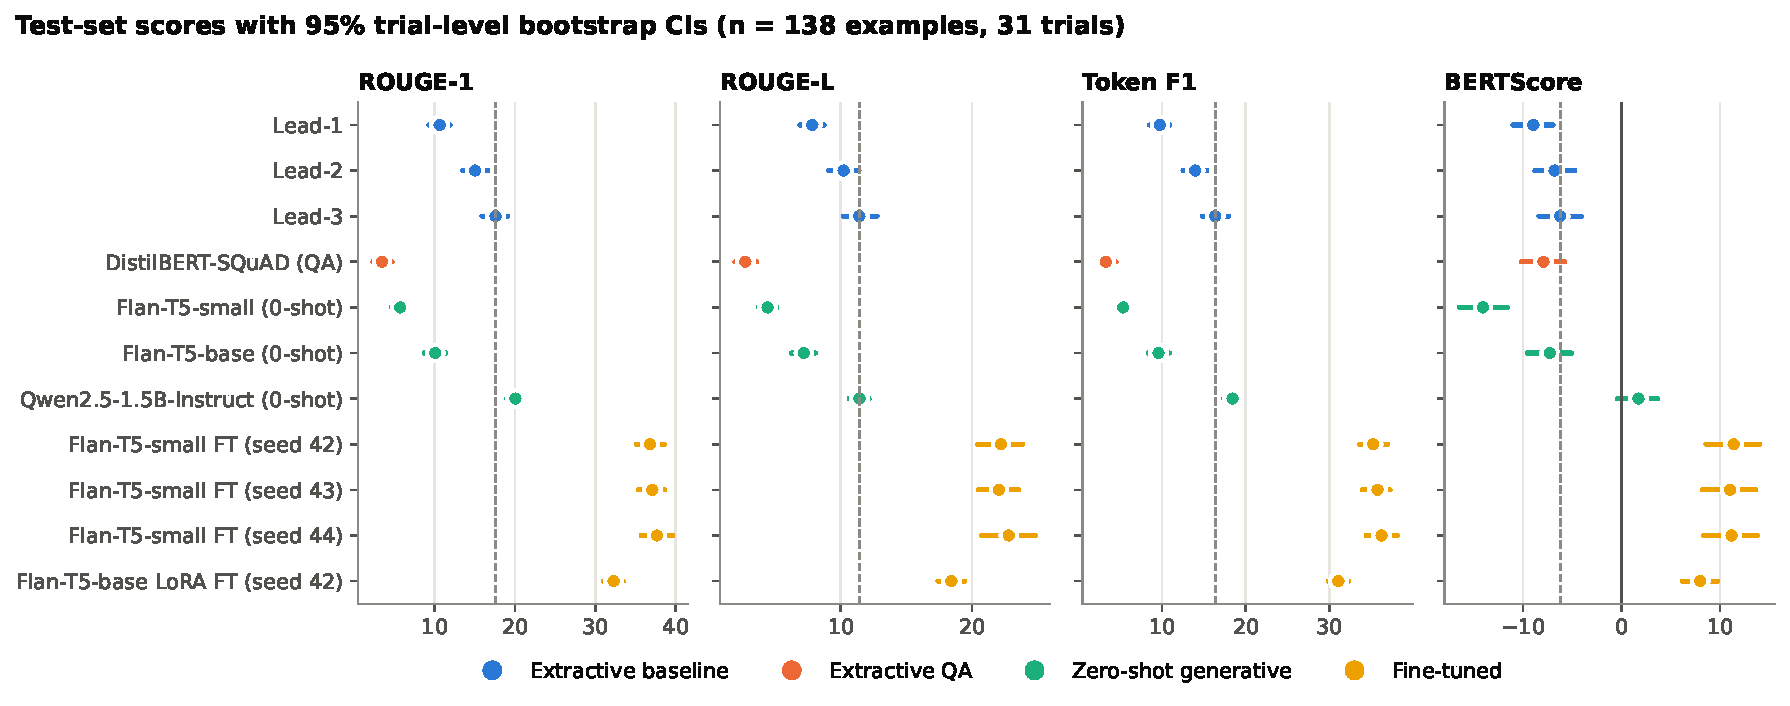
\includegraphics[width=\textwidth]{Figures/results/fig05_main_results_ci.pdf}
    \caption[Main results with confidence intervals]{Test-set scores with 95\% trial-level bootstrap CIs (138 examples, 31 trials). Dashed line: Lead-3.}
    \label{fig:main}
\end{figure}

\paragraph{Fine-tuning dominates on every automatic metric.} After fine-tuning, Flan-T5-small reaches a ROUGE-L of 22.36 $\pm$ 0.39 (mean $\pm$ standard deviation over three seeds), roughly double that of Lead-3 (11.41), the strongest simple baseline. Its BERTScore is 11.21 $\pm$ 0.18, against $-$6.22 for Lead-3. The confidence intervals of the fine-tuned models overlap with no baseline or zero-shot system on any of the metrics shown in Figure~\ref{fig:main}.

\paragraph{Training noise is small.} Table~\ref{tab:seeds} gives the seed variance of fine-tuned Flan-T5-small. The standard deviation across seeds (0.39 ROUGE-L, 0.18 BERTScore) is an order of magnitude smaller than the gaps between system families. Seed variance was measured only for this configuration; the LoRA model has a single seed.

\begin{table}[htbp]
    \centering
    \small
    \caption[Seed variance]{Seed variance of fine-tuned Flan-T5-small (mean $\pm$ standard deviation over seeds 42, 43 and 44).}
    \label{tab:seeds}
    \resizebox{\textwidth}{!}{%
    \begin{tabular}{lrrrrrr}
        \toprule
        System & ROUGE-1 & ROUGE-2 & ROUGE-L & BLEU & Token F1 & BERTScore \\
        \midrule
        \tabinput{Tables/seed_variance_body.tex}
        \bottomrule
    \end{tabular}}
\end{table}

\paragraph{The smaller, fully fine-tuned model beats LoRA on the base model, under our budget.} Flan-T5-base with LoRA reaches a ROUGE-L of 18.43 and a BERTScore of 8.00, below every Flan-T5-small seed. This holds only for our CPU budget: the LoRA run has one seed and its validation loss was still falling after three epochs (Appendix~\ref{sec:training}). It is not evidence that larger models are worse.

\paragraph{Zero-shot systems are weak, and Qwen ties Lead-3 on ROUGE-L.} Qwen2.5-1.5B-Instruct ties Lead-3 on ROUGE-L (11.43 against 11.41) but is clearly ahead on BERTScore (1.73 against $-$6.22): it paraphrases rather than copies, without matching the wording of the references. Zero-shot Flan-T5 scores below Lead-1 on ROUGE-L (4.43 for the small and 7.19 for the base model, against 7.83), largely because its outputs are very short (Section~\ref{sec:length}).

\paragraph{Extractive question answering is the weakest system.} DistilBERT-SQuAD reaches a ROUGE-L of 2.72 and returns an empty answer for 40.6\% of the test examples. Section~\ref{sec:extractive} explains why.

\section{Paired Tests}

Table~\ref{tab:paired} reports the paired comparisons. Every comparison is significant after Holm correction except two. \textbf{Qwen and Lead-3 do not differ on ROUGE-L} (mean difference 0.01 [$-$0.94, 0.84], $p_\text{Holm} = 0.660$) although Qwen is ahead on BERTScore by 7.95 [6.63, 9.19]. \textbf{DistilBERT-SQuAD and Lead-3 do not differ on BERTScore} ($p_\text{Holm} = 0.660$), while DistilBERT is far behind on ROUGE-L. Fine-tuned Flan-T5-small beats Lead-3 by 10.81 [9.61, 12.01] ROUGE-L, scoring higher on 94.2\% of examples, and by 17.61 [15.13, 20.19] BERTScore, scoring higher on 87.0\%. Fine-tuning adds 17.79 ROUGE-L and 25.46 BERTScore to zero-shot Flan-T5-small, and 11.24 and 15.29 to zero-shot Flan-T5-base. Flan-T5-base with LoRA trails fine-tuned Flan-T5-small by 3.79 [2.65, 4.92] ROUGE-L and 3.39 [0.97, 5.48] BERTScore ($p_\text{Holm} = 0.004$).

\begin{table}[htbp]
    \centering
    \footnotesize
    \caption[Paired tests]{Paired comparisons on the 138 test examples. $\Delta$: mean per-example difference (A $-$ B) with 95\% trial-level CI. Win\,\%: share of examples on which A scores higher. $p$: Wilcoxon signed-rank, Holm-corrected over all 20 comparisons. Systems use the main protocol unless marked ``plain greedy''.}
    \label{tab:paired}
    \resizebox{\textwidth}{!}{%
    \begin{tabular}{lrrrrrr}
        \toprule
        & \multicolumn{3}{c}{ROUGE-L} & \multicolumn{3}{c}{BERTScore} \\
        \cmidrule(lr){2-4}\cmidrule(lr){5-7}
        A vs B & $\Delta$ [95\% CI] & Win\,\% & $p$ & $\Delta$ [95\% CI] & Win\,\% & $p$ \\
        \midrule
        \tabinput{Tables/paired_tests_body.tex}
        \bottomrule
    \end{tabular}}
\end{table}

\section{Decoding Ablation}
\label{sec:decoding}

Table~\ref{tab:decoding} and Figure~\ref{fig:decoding} compare plain greedy decoding with the main protocol. The inputs and models are identical; only the decoding rule changes.

\begin{table}[htbp]
    \centering
    \footnotesize
    \caption[Decoding ablation]{Decoding ablation on the test set. PG: plain greedy. NR3: greedy with no-repeat-3 (main protocol). Rep.\,\%: share of outputs with more than 20\% repeated word trigrams. Code and number support: share of codes or numbers in the output found in the context.}
    \label{tab:decoding}
    \resizebox{\textwidth}{!}{%
    \begin{tabular}{lrrrrrrrrrr}
        \toprule
        & \multicolumn{2}{c}{ROUGE-L} & \multicolumn{2}{c}{BERTScore} & \multicolumn{2}{c}{Rep.\,\%} & \multicolumn{2}{c}{Code support} & \multicolumn{2}{c}{Number support} \\
        \cmidrule(lr){2-3}\cmidrule(lr){4-5}\cmidrule(lr){6-7}\cmidrule(lr){8-9}\cmidrule(lr){10-11}
        System & PG & NR3 & PG & NR3 & PG & NR3 & PG & NR3 & PG & NR3 \\
        \midrule
        \tabinput{Tables/decoding_ablation_body.tex}
        \bottomrule
    \end{tabular}}
\end{table}

\begin{figure}[htbp]
    \centering
    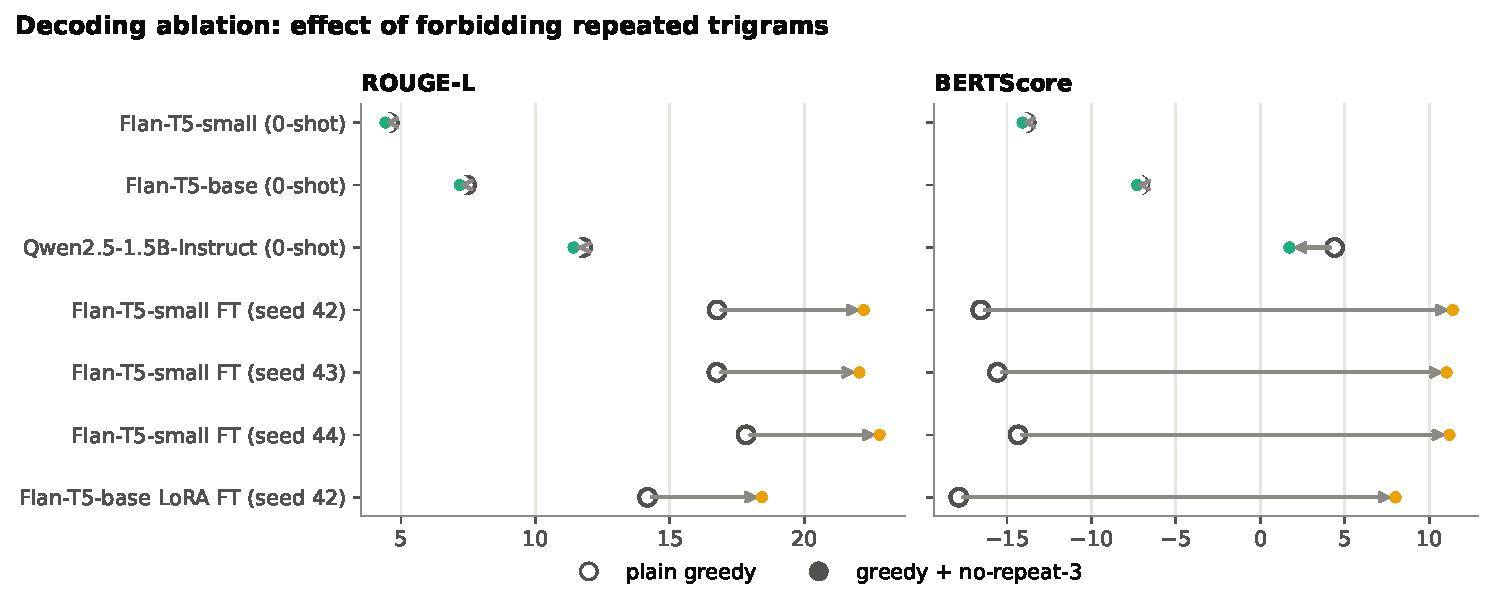
\includegraphics[width=\textwidth]{Figures/results/fig11_decoding_ablation.pdf}
    \caption[Decoding ablation]{Effect of forbidding repeated trigrams (open circle: plain greedy; filled: no-repeat-3).}
    \label{fig:decoding}
\end{figure}

\paragraph{Plain greedy decoding makes the fine-tuned models loop.} Between 86.23\% and 89.13\% of the fine-tuned Flan-T5-small outputs, and 98.55\% of the LoRA outputs, are repetitive. Yet under plain greedy decoding fine-tuned Flan-T5-small (seed 42) still scores a ROUGE-L of 16.76, above Lead-3, while its BERTScore of $-$16.54 is lower than that of every system in the main table. \textbf{ROUGE alone would have reported a working system.} Looping text keeps reusing domain vocabulary that also occurs in the reference, which feeds unigram and longest-common-subsequence overlap.

\paragraph{The no-repeat constraint removes the loops but is not free.} It brings the share of repetitive outputs to 0 and raises BERTScore by 27.94 for fine-tuned Flan-T5-small and 25.85 for LoRA, and ROUGE-L by 5.46 and 4.26 (Table~\ref{tab:paired}). But it also prevents the model from writing the same multi-token drug code twice. Code support of the fine-tuned models falls from 0.95--1.00 under plain greedy decoding to 0.35--0.46: the second mention of a code mutates, for example ACZ885 becomes ACZ855.

\paragraph{Zero-shot models are barely affected,} because they did not loop in the first place. Qwen does slightly better under plain greedy decoding (BERTScore 4.40 against 1.73).

Together with the Qwen and Lead-3 tie, the ablation shows that \textbf{the conclusion a metric supports depends on decoding settings and on the choice of metric}. Decoding settings should be reported as part of the system definition, and overlap metrics should be accompanied by a semantic metric and a repetition check.
